%%%%%%%%%%%%%%%%%%%%%%%%%%%%%%%%%%%%%%%%%%%%%%%%%%%%%%%%%%%%%%%%%%%%%%%%%%%%%%%%
%2345678901234567890123456789012345678901234567890123456789012345678901234567890
%        1         2         3         4         5         6         7         8

\documentclass[letterpaper, 10 pt, conference]{ieeeconf}  % Comment this line out if you need a4paper

%\documentclass[a4paper, 10pt, conference]{ieeeconf}      % Use this line for a4 paper

\IEEEoverridecommandlockouts                              % This command is only needed if 
                                                          % you want to use the \thanks command

\overrideIEEEmargins                                      % Needed to meet printer requirements.

% See the \addtolength command later in the file to balance the column lengths
% on the last page of the document

% The following packages can be found on http:\\www.ctan.org
\usepackage{graphicx} % for pdf, bitmapped graphics files
%\usepackage{epsfig} % for postscript graphics files
%\usepackage{mathptmx} % assumes new font selection scheme installed
%\usepackage{times} % assumes new font selection scheme installed
\usepackage{amsmath} % assumes amsmath package installed
\usepackage{amssymb}  % assumes amsmath package installed
\usepackage{multicol}

\title{\LARGE \bf
Secret Key Generation on a FPGA using a PUF  
}


\author{Justin Cox and Tyler Travis
\\ \small{Department of Electrical and Computer Engineering}
\\ \small{Utah State University}
\\ \small{Logan, Utah 84322}
\\ \small{email: justin.n.cox@gmail.com, tyler.travis@aggiemail.usu.edu}
}

\usepackage{listings}
\usepackage{color}

\definecolor{dkgreen}{rgb}{0,0.6,0}
\definecolor{gray}{rgb}{0.5,0.5,0.5}
\definecolor{mauve}{rgb}{0.58,0,0.82}

\lstset{frame=none,
  language=C,
  aboveskip=3mm,
  belowskip=3mm,
  showstringspaces=false,
  columns=flexible,
  basicstyle={\small\ttfamily},
  numbers=none,
  numberstyle=\tiny\color{gray},
  keywordstyle=\color{blue},
  commentstyle=\color{dkgreen},
  stringstyle=\color{mauve},
  breaklines=true,
  breakatwhitespace=true,
  tabsize=3
}

\begin{document}



\maketitle
\thispagestyle{empty}
\pagestyle{empty}


%%%%%%%%%%%%%%%%%%%%%%%%%%%%%%%%%%%%%%%%%%%%%%%%%%%%%%%%%%%%%%%%%%%%%%%%%%%%%%%%
\begin{abstract}

Encryption has become an important standard for data storage and protection.  In order to encrypt or decrypt the information, a secret key must be used.  This secret key is usually stored somewhere in memory where it potentially can be stolen.  To avoid this, new methods of secret key generation have been developed.  One of these methods is using a Physical Unclonable Function (PUF) to securely generate the secret key.  This paper will cover the design, implementation, and experimental results of a PUF implemented on a FPGA.

\emph{Index Terms}---secret key generation, security, PUF, FPGA.

\end{abstract}

%%%%%%%%%%%%%%%%%%%%%%%%%%%%%%%%%%%%%%%%%%%%%%%%%%%%%%%%%%%%%%%%%%%%%%%%%%%%%%%%
\section{INTRODUCTION}

A lot of research has been done on the use and applications of Physical Unclonable Functions which will be referred to for the remainder of this paper as PUFs.  Some of these applications include, but are not limited to, authentication, secret key generation, true random number generation, and counterfeit chip identification.  This paper will look into the effectiveness of a PUF used for secret key generation.  This PUF will be developed on an FPGA.  The results will be given at the end of the paper.   

\subsection{Previous Work}

A lot of research has been done on PUFs.  More important to this paper, research has been done on improving the reliability and effectivness of PUFs on FPGAs [1].

\subsection{Contribution}

This paper will try to reproduce the PUF designed and analyzed in [1] on a different FPGA.  This paper aims to verify the claims made in the previous work.  Our main contribution is to test the PUF and see if it will work well enough as a secret key generator for the DES algorithm.


%%%%%%%%%%%%%%%%%%%%%%%%%%%%%%%%%%%%%%%%%%%%%%%%%%%%%%%%%%%%%%%%%%%%%%%%%%%%%%%%
\section{OVERVIEW}

\subsection{Data Encryption Standard}

A brief overview of DES will be given so that the reader has a better understanding of how the algorithm works and will better understand where DPA can be used.  If the reader would like an in-depth understanding of DES, it is recommended that the reader look to other sources [2].

The DES algorithm takes a 64-bit plaintext input.  It is then run through an initial permutation that outputs 56-bits which are then split into two halves.  The data goes through sixteen rounds that each have a sub-key that is generated for each round based on the original 64-bit DES key.  After the sixteenth round, the output is run through a finial permutation and the algorithm outputs a 64-bit encrypted ciphertext.  The PUF will be used to generate the 64-bit secret key used to create the subkeys for the sixteen rounds.


\subsection{Physical Unclonable Function}

A Physical Unclonable Function (PUF) is a physical entity used to produce information that can only be reproduced using the same physical device.  Since physical imperfections and deviations are normal in the manufacturing and design process of circuits and devices, each different device of the same family should have different physical characteristics that only pertain to said device.  These imperfections, whether they be voltage levels, temperature, or delay times, can be used to produce information.

PUFs are especially effective when used in security.  Since PUFs are generally difficult to model, the only way an attacker could recover the information generated by the PUF is to steal the actual physical device.  Even then, if the attacker where to inspect the PUF they would risk changing the physical characteristics of the device and the PUF's output may change.

There are many different types of PUFs such as Optical PUFs, Delay PUFs, and SRAM PUFs.  This paper will focus on a design which uses a Delay PUF, more specifically, a type of Arbiter PUF.

%%%%%%%%%%%%%%%%%%%%%%%%%%%%%%%%%%%%%%%%%%%%%%%%%%%%%%%%%%%%%%%%%%%%%%%%%%%%%%%%
\section{PUF DESIGN}

Arbiter PUFs, which will be referred to as APUFs, are a well known delay PUF but they are infamous for having trouble being implemented on FPGAs.  It also has been proven that an APUF can be modeled and simulated allowing an attacker to guess the response message from a given challenge.

There are different variations of the APUF and some of these variations improve the reliability and effectiveness of the APUF.  One variation that has shown improvements is the Double APUF or DAPUF [3].  The DAPUF is made by duplicating a single APUF on an FPGA.  Another variation that has improved the resistance to modeling of an APUF is the XOR APUF [4].  The XOR APUF taks multiple APUFs' output and XORs them together.  This decreases an attackers ability to model the APUF but it requires more APUFs to be built on the FPGA.

As mentioned in [1], the PUF that this paper will be using for secret key generation is the 3-1 DAPUF.  This APUF is a combination of the DAPUF and the XOR APUF.  It duplicates three APUFs on a FPGA and XORs their respective outputs together.  This means that for each response bit, 3 APUFs are needed.  The overall structure of the 3-1 DAPUF is shown in Figure 1.

\begin{figure}[thpb]
	\centering
	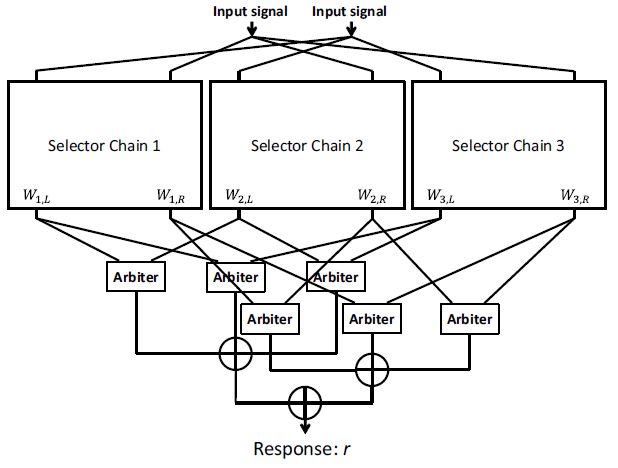
\includegraphics[scale=.50]{DAPUF}
   \caption{3-1 DAPUF figure taken from [1].}
\end{figure}

The APUF is split into three distinct parts.  These three parts are the input signal, the Selector Chain, and the Arbiter.  In order for the reader to better understand the design, the Selector Chain is shown in detail in Figure 2.  The Selector Chain is a chain of MUXes that will either cross the signal or send it straight through.  The travel direction of the signal depends on the challenge bits.  The Selector Chain creates a physical delay.  The outputs of the Selector Chain are sent to an Arbiter which determines which signal arrives first.

\begin{figure}[thpb]
	\centering
	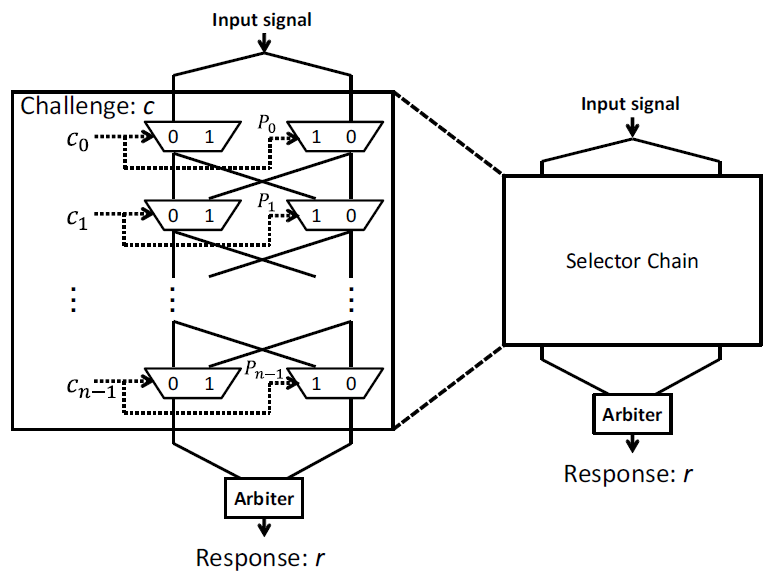
\includegraphics[scale=.42]{Chain}
   \caption{Details of the Selector Chain taken from [1].}
\end{figure}

Normal APUF designs have a difficult time working well on an FPGA because of the problem of symmetry. If the Selector Chains paths are not symmetric, the output will be heavily biased to either a 1 or a 0.  This will make the APUF have a low uniqueness among other APUFs.  The 3-1 DAPUF was designed specifically to work well with FPGAs.  The duplicated APUF needs to be copied to a neighboring SLICE on the FPGA.  Since the duplicated APUF is a copy of the original, the neighboring SLICE should have close to the same wire lengths.  This paper will try to emulate that design using Xilinx ISE and Xilinx Plan Ahead.

\section{SECRET KEY GENERATION}

One of the difficulties of using a PUF for secret key generation is the value of \emph{$\mu$intra}.  The measurement \emph{$\mu$intra} is used to determine how much the output response changes of a certain PUF when given the same input challenge.  Ideally, a PUF should generate the same response when given the same challenge.  Two different PUFs should also generate a different response when given the same challenge.  This measurement is referred to as \emph{$\mu$inter}.  A good PUF should have a \emph{$\mu$inter} close to $50\%$ and a \emph{$\mu$intra} close to $0\%$.

The reason \emph{$\mu$intra} is important is because in a encryption/decryption algorithm, even the slightest change to the secret key will change the cypher-text dramatically.  This means that in order to use a PUF for secret key generation, the PUF's challenge-response pairs need to be consistent.  Since this is almost impossible to do using a PUF, the design of this paper will use Error Correcting Code (ECC) to fix the response output.  A flow chart of this design is shown in Figure 3.

\begin{figure}[thpb]
	\centering
	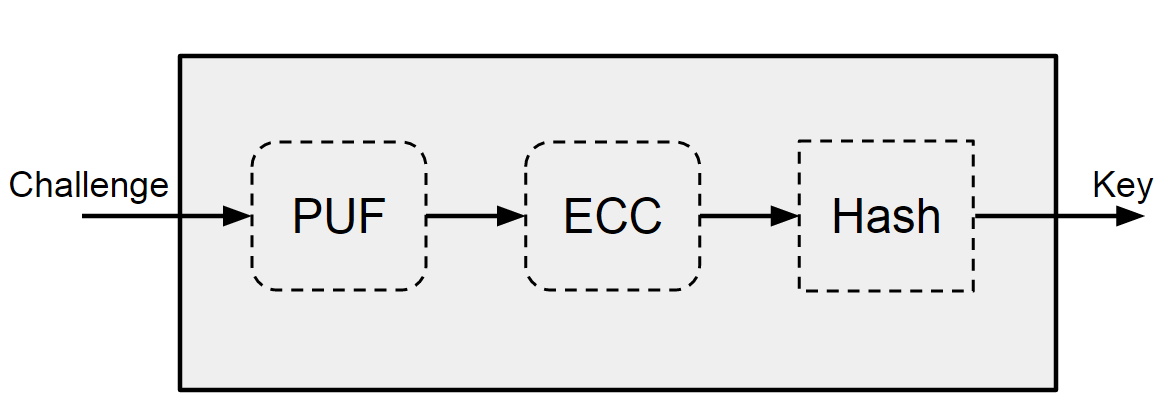
\includegraphics[scale=.25]{keyGen}
   \caption{Flow chart of the secret key generation process.}
\end{figure}

Majority voting will be used to determine what bits of the response output typically change given the same challenge input.  This process is explained in detail in [5], but a brief overview of the process will be given.  A chosen challenge message will be sent through the PUF multiple times.  It will then be determined which bits have a tendency to change.  These bits will be thrown out and the new challenge message will be sent in the ECC.  The ECC encoding process will return parity bits associated with the certain challenge message.  During normal operation, these parity bits will be used to fix the response output for a given challenge.  This process will make sure that the secret key will remain the same for a given challenge.

As shown in Figure 3, it is also a good idea to hash the output from the ECC to inhibit the attacker from knowing the response message.  The design can be made even more secure by adding a hash function to the challenge input as well.  The hash function will not be implemented in this paper's design because the main focus of the paper is to prove that a PUF can be used for secret key generation.  

\section{RESULTS}
 
The 3-1 DAPUF was successfully implemented on a Digilent Nexys 2 FPGA board.  The system clock was running at 50 MHz.  The initial design was planned to have a challenge of 64-bits.  However, the 3-1 DAPUF requires over 20,000 Look Up Tables (LUTs) and the Nexys 2 only has 17,000 LUTs.  As a result of this limitation, a key of 32-bits was chosen.

We tested 10 different challenges 100 times each to measure \emph{$\mu$intra} and \emph{$\mu$inter}.  We also measured \emph{$\mu$intra} at the normal FPGA operating temperature of 85 degrees Fahrenheit and at a hotter temperature of 185 degrees Fahrenheit.  To measure \emph{$\mu$inter}  we ran the same challenge messages on 2 different FPGAs.  Our  \emph{$\mu$intra} at normal temperature was $4.29\%$ and at the hotter temperature it was $7.03\%$.  A slight decrease in the quality of \emph{$\mu$intra} was observed at higher temperatures, but overall it retained good results.  The \emph{$\mu$inter} that we measured was $23.82\%$.  This \emph{$\mu$inter} could be a lot better, but it should be sufficient for secret key generation because the output of the ECC is typically sent through a HASH function.  One reason we achieved a low \emph{$\mu$inter} is because we were not able to enforce symmetry.   This would be fixed in a later revision.
        
A free open source BCH IP core was found on the OpenCores by Ruslan Lepetenok and it was utilized in the design.  The BCH core is able to correct 2 error bits.  In order to make sure that the challenge message has 32 reliable bits, the 3-1 DAPUF for this design produces 40 response bits.  This allows the output response to have 8 bits that can be tossed out after the majority voting.  The BCH core was verified to correct two errors and this can be seen in Figure 4.

\begin{figure}[thpb]
	\centering
	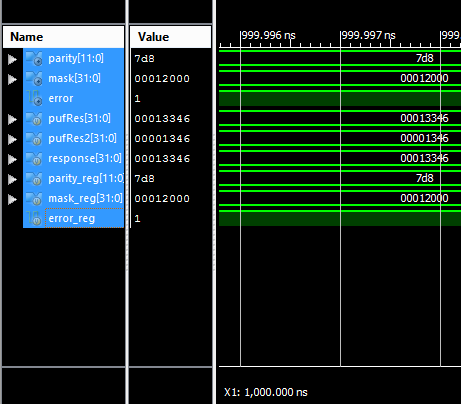
\includegraphics[scale=.75]{bch}
   \caption{\emph{pufRes} is the correct output, \emph{pufRes2} is the output with 2 error bits, and \emph{response} is the corrected output response}
\end{figure}

\section{CONCLUSION}

The teams results were able to reinforce the results found in [1] using the Double Arbiter PUF. The number of slices the DAPUF takes up requires a large number of slices on the FPGA, restricting this design to bigger FPGAs. The team was unable to create a symmetric PUF scheme which would have increased \emph{$\mu$inter} significantly in comparison to our results.

\addtolength{\textheight}{-12cm}   % This command serves to balance the column lengths
                                  % on the last page of the document manually. It shortens
                                  % the textheight of the last page by a suitable amount.
                                  % This command does not take effect until the next page
                                  % so it should come on the page before the last. Make
                                  % sure that you do not shorten the textheight too much.

%%%%%%%%%%%%%%%%%%%%%%%%%%%%%%%%%%%%%%%%%%%%%%%%%%%%%%%%%%%%%%%%%%%%%%%%%%%%%%%%



%%%%%%%%%%%%%%%%%%%%%%%%%%%%%%%%%%%%%%%%%%%%%%%%%%%%%%%%%%%%%%%%%%%%%%%%%%%%%%%%



%%%%%%%%%%%%%%%%%%%%%%%%%%%%%%%%%%%%%%%%%%%%%%%%%%%%%%%%%%%%%%%%%%%%%%%%%%%%%%%%

%\section*{ACKNOWLEDGMENT}

%The author would like to thank his instructor Dr. Rajnikant Sharma %for his help in understanding control concepts.




%%%%%%%%%%%%%%%%%%%%%%%%%%%%%%%%%%%%%%%%%%%%%%%%%%%%%%%%%%%%%%%%%%%%%%%%%%%%%%%%


\begin{thebibliography}{99}

\bibitem{c1} T. Machida, D. Yamamoto, M. Iwamoto, K. Sakiyama. A New Mod of Operation for Arbiter PUF to Improve Uniqueness on FPGA. The University of Electro-Communications. Tokyo, Japan. 2014.
\bibitem{c2} J. Orlin Grabbe. The DES Algorithm Illustrated. \emph{Laissez Faire City Times}, 2006.
\bibitem{c3} T. Machida, D. Yamamoto, M. Iwamoto, K. Sakiyama. Implementation of Double Arbiter PUF and its Performance Evaluation on FPGA. The University of Electro-Communications. Tokyo, Japan. 2015.
\bibitem{c4} M. Rostami, M. Majzoobi, F. Koushanfar, D. Wallach, S. Devadas. Robust and Reverse-Engineering Resilient PUF Authentication and Key-Exchange by Substring Matching. Rice University. Houston, Texas. January. 2014.
\bibitem{c5} Martin Deutschmann. Cryptographic Applications with Physically Unclonable Functions. Alpen-Adria-Universit{\"a}t Klagenfurt. Klagenfurt. November. 2010.

\end{thebibliography}

\end{document}
